\chapter{Implementation}
Here we should talk about bnfc and
alex. What we use from the different programs. How this is useful
is it because of laziness or are the existing solutions good??

\section{Alex}
Alex is a tool for generating lexical analyzers built in Haskell, given a description of the language
in form of regular expressions. The result will be Haskell 98 compatible and can easily be used with the
parser Happy, a parser generator for Haskell.
\subsection{The DFA design}

\section{Monoid}
In abstract algebra a monoid is a set, $S$, and a binary operation $\bullet$ which fulfills the following
three properties:
\begin{description}
\item[Closure] $\forall a,b \in S: a \bullet b \in S$
\item[Associativity] $\forall a,b,c \in S: (a \bullet b) \bullet c = a \bullet (b \bullet c)$
\item[Identity element] $\exists e \in S: \forall a \in S: e \bullet a = a \bullet e = a$
\end{description}

\subsection{The Base case}
\subsection{The Conquer Step}

\section{Fingertree}
The incremental lexer uses a tree structure to save already lexed content.
This tree is of form Fingertree.
What that is and the basics of it is described in this section.

\subsection{Fundamental Concepts}
Before describing the functionality, lets take a look on which building blocks
the fingertrees uses.
\paragraph{First,}
fingertrees uses monoids which has been described earlier in this chapter.
\paragraph{Second,} 
fingertrees uses Right and Left Reductions. This is a function which
collapses a structure of $f$ $a$ into a single value of type $a$. The base case
for when the tree is empty is replaced with a constant value, such as 
$\emptyset$. Intermediate results are combined using a binary operation, like
the monoids $\bullet$. Reduction with a monoid always return the same value,
independent of the argument nesting. But for a reduction with an arbitrary
constant and binary operation there must be a specified nesting rule. If
combining operation are only nested to the right, or to the left, the obtained
result will be a skewed reductions, which can be singled out as a type class.
\lstinputlisting[language=Haskell]{examples/FingerTreeReduceFun.hs}

\subsection{Simple Sequence}
lets take a look on the definition on a 2-3 fingertree and how they can
implement a sequence. Lets start by looking at an ordinary 2-3 tree like in \cref{fig:2-3tree}.
\begin{figure}[!h]
  \centering
\tikzset{
  treenode/.style = {align=center, inner sep=0pt, text centered,
    font=\sffamily},
  branch/.style = {treenode, circle, draw=black, minimum size=0.2cm, text width=0.2em},
  leaf/.style = {treenode, circle, draw=black, font=\sffamily\bfseries, text width=1.5em}
}
    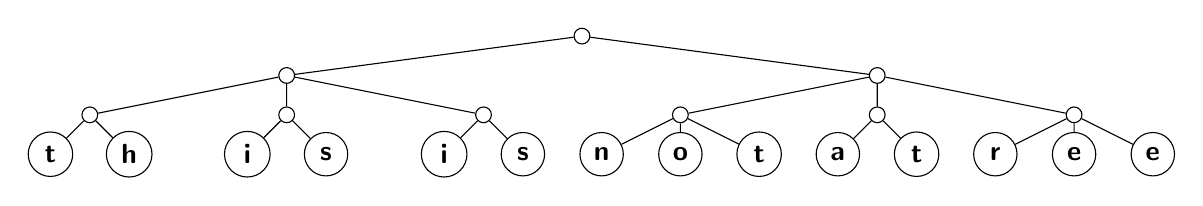
\begin{tikzpicture}[auto,
                        level 1/.style={sibling distance=7.5cm},
                        level 2/.style={sibling distance=2.5cm}, 
                        level 3/.style={sibling distance=1cm},
                        level distance = 0.5cm] 
\node [branch] {}
    child{ node [branch] {}
        child{ node [branch] {}
        	child{ node [leaf] {t}
            }
			child{ node [leaf] {h}
            }
        }
        child{ node [branch] {}
        	child{ node [leaf] {i}
            }
			child{ node [leaf] {s}
            }
        }
        child{ node [branch] {} 
        	child{ node [leaf] {i}
            }
			child{ node [leaf] {s}
            }
        }
    }
    child{ node [branch] {}
        child{ node [branch] {} 
        	child{ node [leaf] {n}
            }
			child{ node [leaf] {o}
            }
			child{ node [leaf] {t}
            }
        }
        child{ node [branch] {} 
        	child{ node [leaf] {a}
            }
			child{ node [leaf] {t}
            }
        }
        child{ node [branch] {} 
        	child{ node [leaf] {r}
            }	
			child{ node [leaf] {e}
            }
			child{ node [leaf] {e}
            }
        } 
    }
; 
\end{tikzpicture}
  \caption{Ordinary 2-3 tree
  \label{fig:2-3tree}}
\end{figure}
In this section the tree will store all data in the leafs. This can be expressed
by defining an non-regular or nested type, as follows:
\lstinputlisting[language=Haskell]{examples/FingerTree2-3Tree.hs}
Operations on these types of trees usually takes logarithmic time in the size of
the tree. But for sequence representations a constant time complexity is
preferable for adding or removing element from the start or end of the sequence.

A finger is a structure which provides efficient access to nodes near the
distinguished location. To obtain efficient access to the start and end of the
sequence represented by the tree, there should be fingers placed at the left and
right end of the tree. In the example tree, taking hold of the end nodes of and
lifting them up together. The result should look like in \cref{fig:fingertree}
\begin{figure}[!h]
  \centering
  \tikzset{
  treenode/.style = {align=center, inner sep=0pt, text centered,
    font=\sffamily},
  branch/.style = {treenode, circle, draw=black, minimum size=0.2cm, text width=0.2em},
  blackbranch/.style = {treenode, draw,fill=black!33, minimum size=0.2cm, text width=0.2em},
  leaf/.style = {treenode, circle, draw=black, font=\sffamily\bfseries, text width=1.5em}
}
    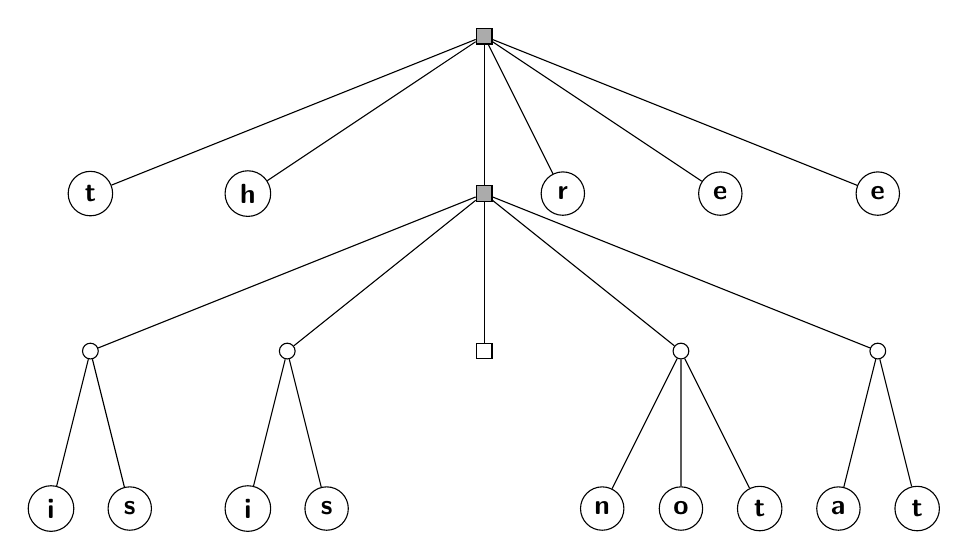
\begin{tikzpicture}[level distance=2cm, sibling distance = 2cm]
    \node[blackbranch] {} 
        child { node[leaf] {t} }
        child { node[leaf] {h} }
        child[level distance=2cm, sibling distance=2.5cm, grow=down] { node[blackbranch] {} [level distance=2cm]
            child { node[branch] {} [sibling distance=1cm]
                child { node[leaf] {i} }
                child { node[leaf] {s} }
            }            
            child { node[branch] {} [sibling distance=1cm]
                child { node[leaf] {i} }
                child { node[leaf] {s} }
            }
            child[level distance=2cm, grow=down] { node[blackbranch, fill=white] {}}
            child { node[branch] {} [sibling distance=1cm]
                child { node[leaf] {n} }
                child { node[leaf] {o} }
                child { node[leaf] {t} }
            }
            child { node[branch] {} [sibling distance=1cm]
                child { node[leaf] {a} }
                child { node[leaf] {t} }
            }
        }
        child { node[leaf] {r} }
        child { node[leaf] {e} }
        child { node[leaf] {e} }
    ;
  \end{tikzpicture} 
  \caption{2-3 Fingertree
  \label{fig:fingertree}}
\end{figure}

Since all leafs in the 2-3 tree where at the same level, the left and right
spine has the same length. Therefor the left and right spines can be pair up to
create a single central spine. Branching out from the spine is 2-3 trees. At the
top level there are two to three elements on each side, while the other levels
have one or two sub-trees, whose depth increases down the spine. Depending on if
the root node had 2 or 3 branches in the original 2-3 tree, will the bottom node
either have a single 2-3 tree or empty. This structure can be described as
follows:
\lstinputlisting[language=Haskell]{examples/HaskellFingerTree.hs}
Where Digit is a buffer of elements stored left to right, here represented as a
list for simplicity

The non-regular definition of the $FingerTree$ type determines the unusual shape
of these trees, which is the key to there performance. The top level of the tree
contains elements of type $a$. Next level contains elements of type $Node$ $a$.
At the $n$th level, elements are of type $Node^n$ $a$. which are 2-3 trees with
a depth of $n$. This will give that a sequence of $n$ elements is represented by
a $FingerTree$ of depth $\Theta(\log n)$. Also an element at position $d$ from
the nearest end is stored at a depth of $\Theta(\log d)$ in the $FingerTree$
\cite{fingertree}

In fingertrees and nodes the reduce function mentioned in fundamental concepts
will be generic defined to the following types. 
Reduction for the node:
\lstinputlisting[language=Haskell]{examples/FingerTreeReduceNode.hs}
Reduction of fingertrees single and double lifting of the binary operation:
\lstinputlisting[language=Haskell]{examples/FingerTreeReduceFingerTree.hs}

\subsection{Double-ended Queue Operations}
After showing how the Fingertrees basic structure is defined. It is now time to
show how fingertrees makes efficient Double-ended Queue, a queue structure which
can be accessed from both ends, where all operations having the time complexity
$\Theta(1)$.

Adding a element to the beginning of the sequence is strait forward, except when
the initial buffer ($Digit$) already is full. In this case, push all but one of
the elements in the buffer as a node, leaving behind two elements in the buffer:
\lstinputlisting[language=Haskell]{examples/FingerTreeInfixr.hs}
Adding to the end of the sequence is a mirror image of the above:
\lstinputlisting[language=Haskell]{examples/FingerTreeInfixl.hs}

A insertion operation the basic 2-3 tree, where the data is stored in the leafs,
is done with a time complexity of $\Theta \log n$. In the fingertree the
expected time complexity can be argued in the following way. Digits of two or
three elements (which is isomorphic to elements of type $Node$ $a$) is
classified as safe and those of one or four elements is classified as dangerous.
A double-ended queue operation can only propagate to the next level from a
dangerous element. By doing so making that dangerous element safe, which means
that the next operation reaching that digit will not propagate. This will result
in that at most half of the operations descend one level, at most 1 quarter two
levels, and so on. This will give that in a sequence of operations the average
cost is constant.

The same bound hold in a persisted setting if subtrees are suspended using lazy
evaluation. Laziness makes sure that changes deep in the spine do not take place
until a subsequent operation need to go that far. By the above properties
of safe and dangerous digits, by that time enough cheap shallow operations
will have been performed to pay for the more expensive operation \cite{fingertree}.

\subsubsection{The Bankers Method}
The bankers method accounts for accumulated debt. Each debit represents
a constant amount of suspended work. When a computation initially suspends, it
create a number of debits proportional to it's shared cost and
associate each debit with a location in the object. The choice of location for
each debit depends on the nature of the computation. If the computation is
monolithic (i.e., once begun, it runs to completion), then all debits are
usually assigned to the root of the result, which the incremental lexer is not. 
But if the computation is like the lexer a incremental, then the debits may be 
distributed among the roots of the partial results.

The amortized cost of an operation is the unshared cost of the operation
plus the number of debits discharged by the operation. Note that the number
of debits created by an operation is not included in its amortized cost. The
order in which debits should be discharged depends on how the object will
be accessed; debits on nodes likely to be accessed soon should be discharged
first.

Incremental functions play an important role in the bankers method because
they allow debits to be dispersed to different locations in a data structure,
each corresponding to a nested suspension. Then, each location can be accessed
as soon as its debits are discharged, without waiting for the debits at other
locations to be discharged. This means that the initial partial results of
an incremental computation can be paid for very quickly, and that subsequent
partial results may be paid for as they are needed \cite{Okasaki1999}.

\subsubsection{Banker Method on the Fingertree}
The argument for the amortized time can be expressed using the Banker method.
This is done by assigning the suspension of the middle tree in each Deep node
as many debits as the node has safe digits. (0,1 or 2) A double-ended queue
operation which descends $k$ levels turns $k$ dangerous digits into safe digits.
By doing so creates $k$ debits to pay for the work done.
Applying the bankers method of debit passing to any debits already attached to
these $k$ nodes. It can be showed that each operation must discharge at most
one debit. Therefore the double-ended queue operations run in $\Theta(1)$
amortized time \cite{fingertree}.

\subsection{Concatenation Operations}
Concatenation is a simple operation for most cases, except for the case when two $Deep$ trees are being concatenated. Concatenating with a $Empty$ will be an identity and with a $Single$ will reduce to $<|$ or $|>$. For the hard part when there are two $Deep$ trees, the prefix of the first tree will be the final prefix. Suffix of the second tree will be the suffix of the final tree. The recursive function $app3$ combines two trees and a list of $Nodes$ (basically the old prefix and suffixes down the spines of the old trees):

\lstinputlisting[language=Haskell]{examples/FingerTreeApp3.hs}

Where $(<|')$ and $(|>')$ are the functions defined in the previous sub-section and $nodes$ groups a list of elements into $Node$s: 

\lstinputlisting[language=Haskell]{examples/FingerTreeNodesFunc.hs}

Now to concatenation of the Fingertrees, just call on $app3$ with an empty list between the two trees.

\lstinputlisting[language=Haskell]{examples/FingerTreeConcatFunc.hs}

The time spent on concatenation can be reasoned in this way. Each invocation of $app3$ arising from $(><)$ the argument list has a length of at most 4, which means that each of these invocations takes $\Theta(1)$ time. The recursion terminates when the bottom of the shallower tree has been reached, with up to 4 insertions. So the total time complexity id $\Theta(\log min\{n_1, n_2\})$ where $n_1$ and $n_2$ are the number of elements in the two trees. 

\section{Sequences}
A sequence in Haskell is a form of sophisticated list. That is a list with better performance than the basic [] list notation. Where a list in Haskell has $\Theta(n)$ for finding, inserting or deleting elements, that is in a list there is only known current element and the rest of the list. Which will result in for example finding the last element of a list, the computer must look at every element until the empty list has been found as the rest of the list. Where in a sequence the last element can be obtained in $\Theta(1)$ time. Adding a element anywhere in the sequence can be done in worst case, $\Theta(log n)$ \cite{fingertree}. 

Since this project is about creating as real-time lexing tool, performance is very important. String in Haskell are just a list of characters, [Char], and therefor has $\Theta(n)$ in time cost. Lexing is working with strings in a high frequency and there for there is a idea of instead define a string as a sequence of characters instead of a list of character. 

\section{Fingertree}
The implementation
\section{Transition Map}
\subsection{Array Format}
\subsection{Function Composition Format}
